\documentclass[a4paper]{scrartcl}

\usepackage{float}
\usepackage{tikz}
\usetikzlibrary{arrows,automata}
\usepackage{pgf}
\usepackage[utf8]{inputenc} % this is needed for umlauts
\usepackage[ngerman]{babel} % this is needed for umlauts
\usepackage[T1]{fontenc}    % this is needed for correct output of umlauts in pd
\usepackage{amssymb}
\usepackage{amsmath}
\usepackage{mathrsfs}
\usepackage{dsfont}
\usepackage{graphicx}
\usepackage{fancyhdr}
\usepackage{lastpage}
\usepackage{imakeidx}
\setlength{\parskip}{\medskipamount}
\setlength{\parindent}{0pt}
\usepackage{enumitem}
\usepackage{hyperref}
\usepackage{verbatim}

%%%%%%%%%%%%%%%%%%%%%%%%
% Kopf- und Fusszeilen %
%%%%%%%%%%%%%%%%%%%%%%%%
\pagestyle{fancy}
\lhead{
        Maximilian Roth
}
\chead{Logik-Tutorat Lösungen Blatt 3\\}
\rhead{
        \today{} \\
        Seite \thepage{} von \pageref{LastPage}\\
        
}
\lfoot{}
\cfoot{}
\rfoot{} 

%%%%%%%%%%%%%%%%%%%%%%%%
% Anfang des Dokuments %
%%%%%%%%%%%%%%%%%%%%%%%%

\begin{document}
\section*{Disclaimer}%
\label{sec:disclaimer}
Auch in diesem Dokument können sich Fehler befinden!\\
Sie sind nicht die Musterlösung der Aufgaben, sondern selbst erstellte Lösungen.\\

Als generelle Lektüre kann ich nur das Skript von Markus Junker aus dem WS 17/18 empfehlen:\\
\url{http://home.mathematik.uni-freiburg.de/junker/skripte/InfoLogik.pdf}\\
Hier ist vieles sehr genau und verständlich erklärt.

\section*{}%
\label{sec:aufgabe_1}

    \begin{figure}[H]
        \centering
        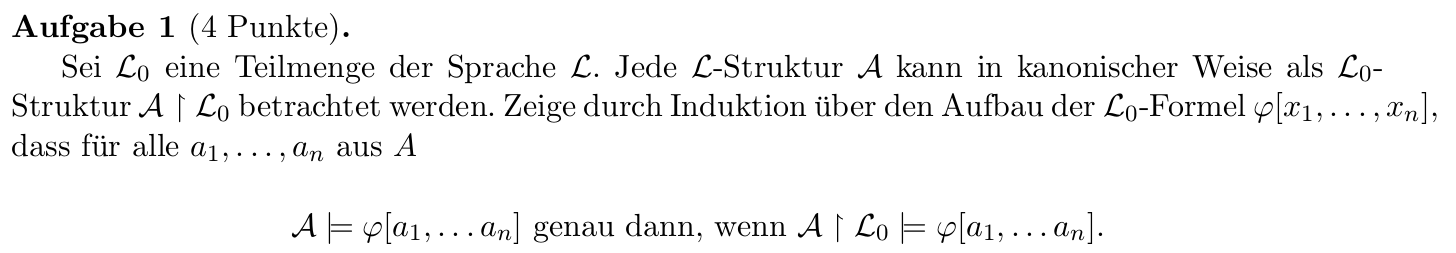
\includegraphics[scale=0.3]{./A-1.png}
        \label{fig:}
    \end{figure}

    \underline{ZZ:} $\mathfrak{A} \vDash \varphi[a_1,\dots,a_n] \Leftrightarrow \mathfrak{A} \upharpoonright \mathscr{L}_0 \vDash \varphi[a_1,\dots,a_n]$\\
    \\\underline{Beweis:}\\
        Zunächst nennen wir $\mathfrak{A} \upharpoonright \mathscr{L}_0$ im Folgenden $\mathfrak{B}$
        Wir machen eine Induktion über den Formelaufbau (wie üblich zeigen wir nur den Induktionsschritt).\\

        \begin{itemize}
            \item Terme:\\
                \begin{itemize}
                    \item $t = c$\\
                        $t^{\mathfrak{A}}[a_1,\dots,a_n] = c = t^{\mathfrak{B}}[a_1,\dots,a_n]$\\
                    \item $t = x_i$\\
                        $t^{\mathfrak{A}}[a_1,\dots,a_n] = x_i = t^{\mathfrak{B}}[a_1,\dots,a_n]$\\
                    \item $t = f(t_1,\dots,t_n)$
                        $t^{\mathfrak{A}}[a_1,\dots,a_n] = f^{\mathfrak{A}}(t_1^{\mathfrak{A}},\dots,t_n^{\mathfrak{A}})
                        \overset{I.V.}{=} f^{\mathfrak{A}}(t_1^{\mathfrak{B}},\dots,t_n^{\mathfrak{B}})
                        = f^{\mathfrak{B}}(t_1^{\mathfrak{B}},\dots,t_n^{\mathfrak{B}})$
                \end{itemize}

\newpage

            \item atomare Formeln:\\
                \begin{itemize}
                    \item $\varphi = t_1 \doteq t_2$\\
                        $\mathfrak{A} \vDash \varphi[a_1,\dots,a_n] \Leftrightarrow t_1^{\mathfrak{A}}[a_1,\dots,a_n] \doteq t_1^{\mathfrak{A}}[a_1,\dots,a_n]\\
                        \Leftrightarrow t_1^{\mathfrak{B}}[a_1,\dots,a_n] \doteq t_1^{\mathfrak{B}}[a_1,\dots,a_n]
                        \Leftrightarrow \mathfrak{B} \vDash \varphi[a_1,\dots,a_n]$\\
                    \item $\varphi = R(t_1,\dots,t_n)$\\
                        $\mathfrak{A} \vDash \varphi[a_1,\dots,a_n] \Leftrightarrow (t_1^{\mathfrak{A}},\dots,t_n^{\mathfrak{A}}) \in R^{\mathfrak{A}}\\
                        \Leftrightarrow (t_1^{\mathfrak{B}},\dots,t_n^{\mathfrak{B}}) \in R^{\mathfrak{A}}
                        \Leftrightarrow (t_1^{\mathfrak{B}},\dots,t_n^{\mathfrak{B}}) \in R^{\mathfrak{B}}
                        \Leftrightarrow \mathfrak{B} \vDash \varphi[a_1,\dots,a_n]$\\
                \end{itemize}

            \item quantorenfreie Formeln:\\
                \begin{itemize}
                    \item $\varphi = \neg \psi$\\
                        $\mathfrak{A} \vDash \varphi[a_1,\dots,a_n] \Leftrightarrow \mathfrak{A} \nvDash \psi[a_1,\dots,a_n]
                        \overset{I.V.}{\Leftrightarrow} \mathfrak{B} \nvDash \psi[a_1,\dots,a_n] \Leftrightarrow \mathfrak{B} \vDash \varphi[a_1,\dots,a_n]$
                    \item $\varphi = \psi_1 \lor \psi_2$\\
                        $\mathfrak{A} \vDash \varphi[a_1,\dots,a_n]\\
                        \Leftrightarrow \mathfrak{A} \vDash \psi_1[a_1,\dots,a_n] \text{ oder } \mathfrak{A} \vDash \psi_2[a_1,\dots,a_n]\\
                        \overset{I.V.}{\Leftrightarrow} \mathfrak{B} \vDash \psi_1[a_1,\dots,a_n] \text{ oder } \mathfrak{B} \vDash \psi_2[a_1,\dots,a_n]\\
                        \Leftrightarrow \mathfrak{B} \vDash \varphi[a_1,\dots,a_n]$\\
                \end{itemize}

            \item Formeln mit Quantoren:\\
                \begin{itemize}
                    \item $\varphi = \exists \psi$\\
                        $\mathfrak{A} \vDash \varphi[a_1,\dots,a_n]\\
                        \Leftrightarrow \mathfrak{A} \vDash \psi[a_1,\dots,a_n,a]\\
                        \overset{I.V.}{\Leftrightarrow} \mathfrak{B} \vDash \psi[a_1,\dots,a_n,a]\\
                        \mathfrak{B} \vDash \varphi[a_1,\dots,a_n]$\\
                \end{itemize}
                        
        \end{itemize}

\section*{}%
\label{sec:aufgabe_2}

    \begin{figure}[H]
        \centering
        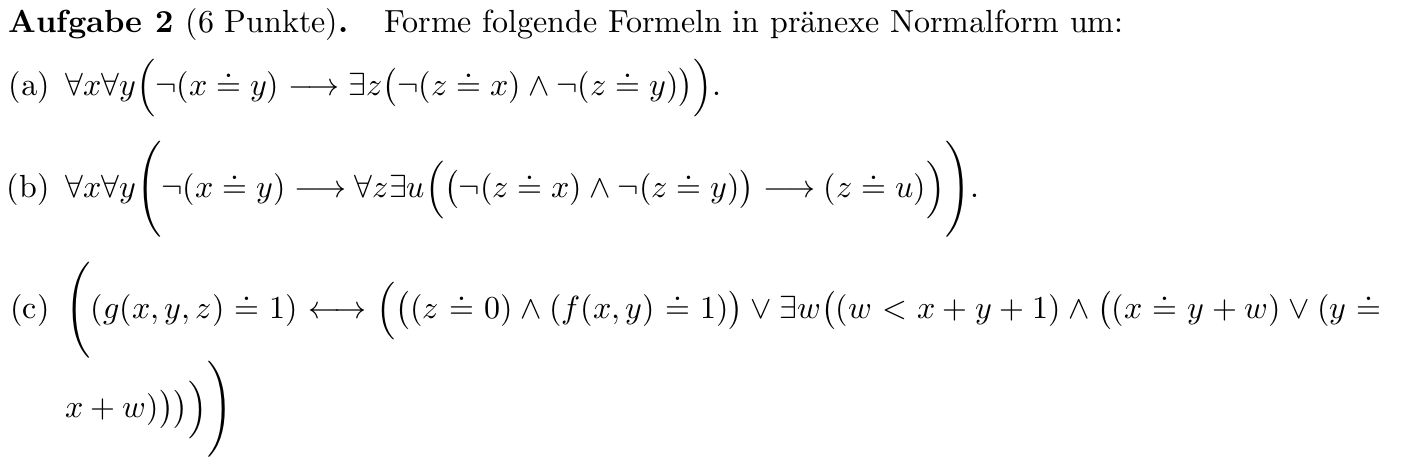
\includegraphics[scale=0.3]{./A-2.png}
        \label{fig:}
    \end{figure}

    \begin{itemize}
        \item a)\\
            $\forall x \forall y (\neg x \doteq y \rightarrow \exists z (\neg z \doteq x \land \neg x \doteq y))$\\
            $\sim \forall x \forall y (x \doteq y \lor \exists z (\neg z \doteq x \land \neg x \doteq y))$\\
            $\sim \forall x \forall y \exists z (x \doteq y \lor (\neg z \doteq x \land \neg x \doteq y))$\\

        \item b)\\
            $\forall x \forall y (\neg x \doteq y \rightarrow \forall z \exists u ((\neg z \doteq x \land \neg z \doteq y) \rightarrow z \doteq u))$\\
            $\sim \forall x \forall y (x \doteq y \lor \forall z \exists u ((\neg z \doteq x \land \neg z \doteq y) \rightarrow z \doteq u))$\\
            $\sim \forall x \forall y \forall z \exists u (x \doteq y \lor ((\neg z \doteq x \land \neg z \doteq y) \rightarrow z \doteq u))$\\

        \item c)\\
            $(gxyz \doteq 1 \leftrightarrow ((z \doteq 0 \land fxy \doteq 1) \lor \exists w (w < x + y + 1 \land (x \doteq y + w \lor y \doteq x + w))))$\\
            \\$\sim ((gxyz \doteq 1 \rightarrow ((z \doteq 0 \land fxy \doteq 1) \lor \exists w (w < x + y + 1 \land (x \doteq y + w \lor y \doteq x + w))))
            \land (((z \doteq 0 \land fxy \doteq 1) \lor \exists w (w < x + y + 1 \land (x \doteq y + w \lor y \doteq x + w))) \rightarrow gxyz \doteq 1))$\\
            \\$\sim ((\neg gxyz \doteq 1 \lor ((z \doteq 0 \land fxy \doteq 1) \lor \exists w (w < x + y + 1 \land (x \doteq y + w \lor y \doteq x + w))))
            \land (\neg((z \doteq 0 \land fxy \doteq 1) \lor \exists w (w < x + y + 1 \land (x \doteq y + w \lor y \doteq x + w))) \lor gxyz \doteq 1))$\\
            \\$\sim \exists w ((\neg gxyz \doteq 1 \lor ((z \doteq 0 \land fxy \doteq 1) \lor (w < x + y + 1 \land (x \doteq y + w \lor y \doteq x + w))))
            \land (\neg((z \doteq 0 \land fxy \doteq 1) \lor \exists w (w < x + y + 1 \land (x \doteq y + w \lor y \doteq x + w))) \lor gxyz \doteq 1))$\\
            \\$\sim \exists w ((\neg gxyz \doteq 1 \lor ((z \doteq 0 \land fxy \doteq 1) \lor (w < x + y + 1 \land (x \doteq y + w \lor y \doteq x + w))))
            \land (\neg \exists w((z \doteq 0 \land fxy \doteq 1) \lor (w < x + y + 1 \land (x \doteq y + w \lor y \doteq x + w))) \lor gxyz \doteq 1))$\\
            \\$\sim \exists w ((\neg gxyz \doteq 1 \lor ((z \doteq 0 \land fxy \doteq 1) \lor (w < x + y + 1 \land (x \doteq y + w \lor y \doteq x + w))))
            \land (\forall w \neg ((z \doteq 0 \land fxy \doteq 1) \lor (w < x + y + 1 \land (x \doteq y + w \lor y \doteq x + w))) \lor gxyz \doteq 1))$\\
            \\$\sim \exists w \forall v((\neg gxyz \doteq 1 \lor ((z \doteq 0 \land fxy \doteq 1) \lor (w < x + y + 1 \land (x \doteq y + w \lor y \doteq x + w))))
            \land (\neg ((z \doteq 0 \land fxy \doteq 1) \lor (v < x + y + 1 \land (x \doteq y + v \lor y \doteq x + v))) \lor gxyz \doteq 1))$\\


    \end{itemize}

\newpage

\section*{}%
\label{sec:aufgabe_3}

    \begin{figure}[H]
        \centering
        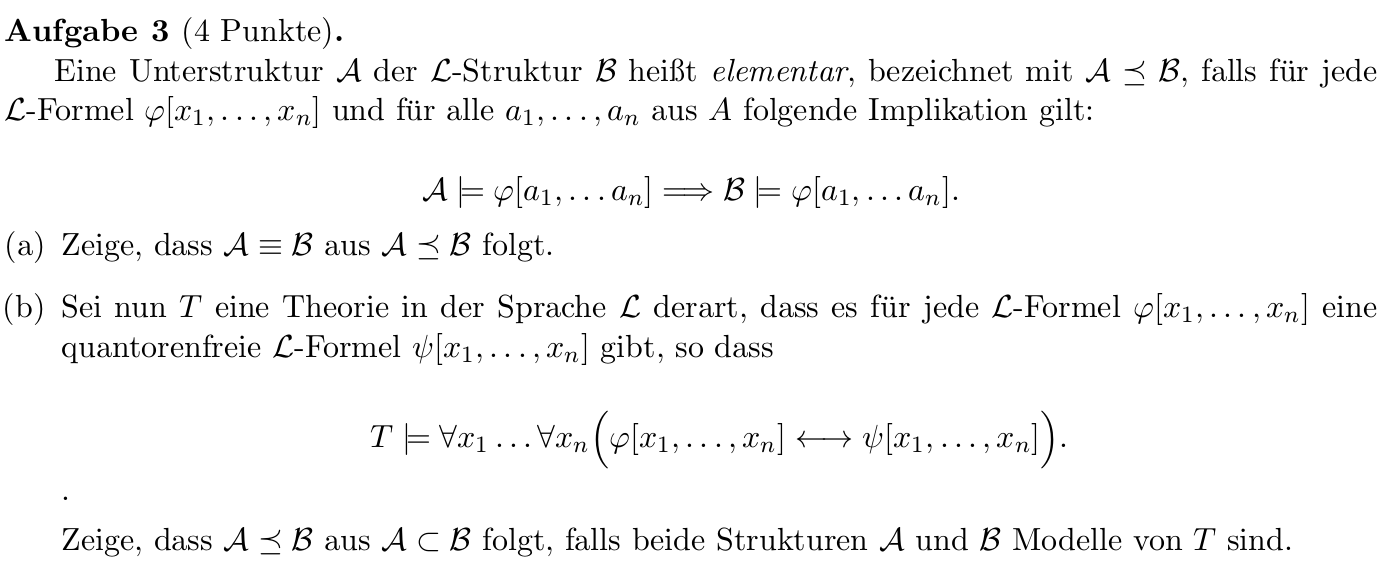
\includegraphics[scale=0.3]{./A-3.png}
        \label{fig:}
    \end{figure}

    \begin{itemize}
        \item a)\\
            \underline{ZZ:} $\mathfrak{A} \preceq \mathfrak{B} \Rightarrow \mathfrak{A} \equiv \mathfrak{B}$\\
            \underline{Bew:}\\
               \begin{figure}[H]
                   \centering
                   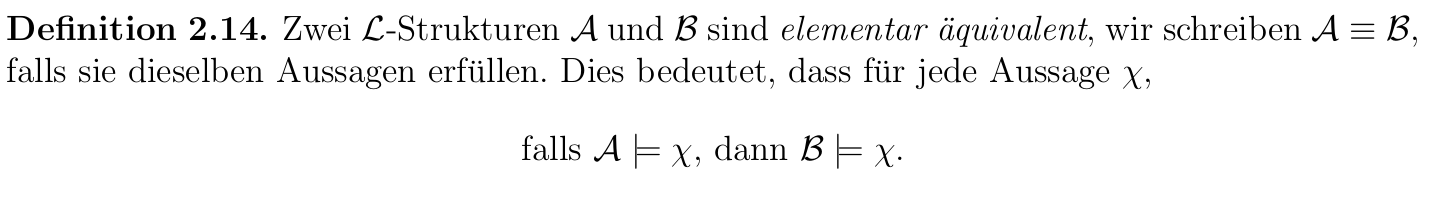
\includegraphics[scale=0.25]{./El-equiv.png}
                   \label{fig:}
               \end{figure} 

               Da die $\mathscr{L}$-Aussagen eine Teilmenge der $\mathscr{L}$-Formeln ist folgt $\mathfrak{A} \equiv \mathfrak{B}$.\\

        \item b)\\
            \underline{ZZ:} Sei $\mathfrak{A} \vDash T, \mathfrak{B} \vDash T, \mathfrak{A} \subset \mathfrak{B}$ dann folgt $\mathfrak{A} \preceq \mathfrak{B}$\\
            \underline{Beweis:}\\
                Für alle $\mathscr{L}$-Formeln $\varphi$ und alle $a_i \in A$ soll also gelten:\\
                $\mathfrak{A} \vDash \varphi[a_1,\dots,a_n] \Rightarrow \mathfrak{B} \vDash \varphi[a_i,\dots,a_n]$\\
                \\Mit T folgt:\\
                $\Leftrightarrow \mathfrak{A} \vDash \psi[a_1,\dots,a_n] \Rightarrow \mathfrak{B} \vDash \psi[a_i,\dots,a_n]$\\
                \\Aus Blatt 3 Aufgabe 4 b) folgt obiges mit quantorenfreiem $\psi \text{ und } \mathfrak{A} \subset \mathfrak{B}$\\
                \\$\Rightarrow \mathfrak{B} \vDash \varphi[a_1,\dots,a_n] \Rightarrow \mathfrak{A} \preceq \mathfrak{B}$\\

    \end{itemize}

\section*{}%
\label{sec:aufgabe_4}

    \begin{figure}[H]
        \centering
        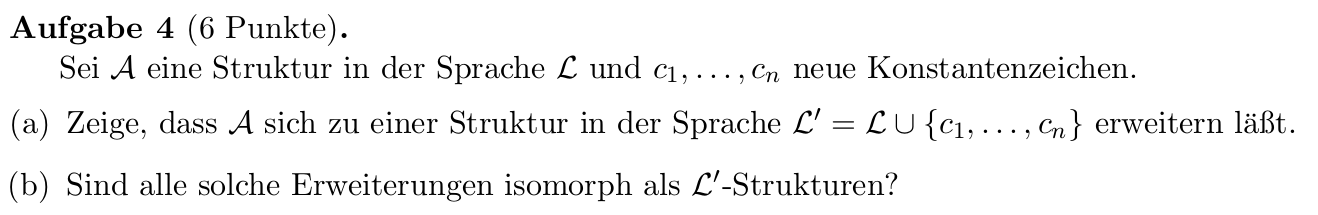
\includegraphics[scale=0.3]{./A-4-1.png}
        \label{fig:}
    \end{figure}

    \begin{figure}[H]
        \centering
        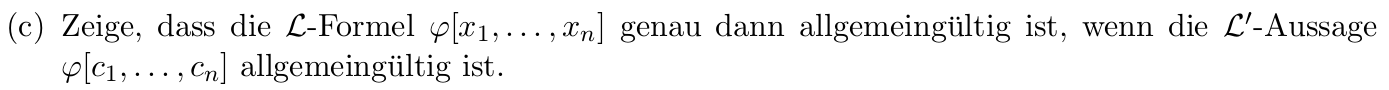
\includegraphics[scale=0.3]{./A-4-2.png}
        \label{fig:}
    \end{figure}

    \begin{itemize}
        \item a)\\
            Sei $a \in A$, dann gilt mit $c_i^{\mathfrak{A'}} = a, \forall i \in \{1,\dots,n\}$,\\
            dass $\mathfrak{A'} = (A, \mathscr{L}') \quad \mathscr{L}'$-Struktur ist.\\ 

        \item b)\\
            Nein, wir beweisen mit Gegenbeispiel.\\
            Sei $\mathfrak{A}' = (A, \mathscr{L}')$ mit $c_i^{\mathfrak{A}'} = a, \forall i \in \{1,\dots,n\}, a \in A$\\
            und Sei $\mathfrak{A}'' = (A, \mathscr{L}')$ mit $c_i^{\mathfrak{A}''} = a_i, \forall i \in \{1,\dots,n\}, a_i \in A \text{ und } a_i \neq a_j
            \text{ für  } i \neq j$\\
            Es gilt: $\mathfrak{A}' \vdash c_i \doteq c_j \text{, aber } \mathfrak{A}'' \nvdash c_i \doteq c_j \text{ für } i \neq j$\\
            $\Rightarrow \mathfrak{A} \text{ und } \mathfrak{B}$ sind nicht isomorph.

        \item c)\\
            \underline{ZZ:} $\vdash \varphi[x_1,\dots,x_n] \Rightarrow \vdash \varphi[c_1,\dots,c_n]$\\
            \\\underline{Beweis:}\\
                Wenn $\varphi[x_1,\dots,x_n]$ allgemeingültig ist, dann ist die Auswertung von den $c_i$ egal, da $\varphi$ für jeden Wert wahr ist.\\
                $\Rightarrow \vdash \varphi[c_1,\dots,c_n]$\\
                \\Wenn $\varphi[x_1,\dots,x_n]$ nicht allgemeingültig ist, dann gibt es $x_1,\dots,x_n$ für die $\varphi$ falsch wird.\\
                Setzen wir nun $c_i^{\mathfrak{A}'} = x_i$, dann ist $\varphi[c_1,\dots,c_n]$ ebenso falsch und kann damit nicht allgemeingültig sein.\\
                

    \end{itemize}

\end{document}
